\documentclass[../Main/Main.tex]{subfiles}

\begin{document}
% Qué? (Objetivo)
En luz de las nuevas y populares tendencias en el mundo de la estadística computacional, llamada en ocasiones aprendizaje estadístico o aprendizaje de máquina;\footnote{\textit{Machine Learning (ML) en la mayoría de la literatura.}} este trabajo plantea como objetivo: estudiar, explicar e implementar un modelo de clasificación supervisada con base en la extensión del modelo \textit{probit} al que se le añade un componente no lineal de bases aditivas en covariables. Asimismo, se desarrolla un algoritmo asociado de aprendizaje para la inferencia del modelo y generación de predicciones con base en el paradigma bayesiano.\footnote{Es común, hacer una distinción entre el aprendizaje estadístico y el aprendizaje de máquina pues, mientras que los modelos son los mismos, difieren en perspectiva. El aprendizaje estadístico presta mayor atención al aspecto inferencial e interpretación, cuando el aprendizaje de máquina coloca mayor énfasis en la implementación computacional y los resultados.}

% Por qué? 
El modelo hace inferencia sobre un conjunto de datos y \textit{aprende} acerca de los patrones subyacentes que estos mismos puedan contener para posteriormente, predecir el resultado de las variables de respuesta. Este tipo de modelos, han resultado ser de enorme efectividad en ámbitos tan diversos, como lo son la medicina y las finanzas. Bajo esta óptica, se busca que el modelo sea práctico y útil, sin perder de vista el componente teórico que lo sustenta. Por lo tanto, se busca explicar a detalle cada componente del modelo y del algoritmo para que éste no sea tratado como una caja negra computarizada.

Los modelos probit son un tipo de regresiones generalizadas, que buscan explicar la clasificación de variables de respuesta $y_i$ binarias (éxito o fracaso, positivo o negativo, etcétera) con base en un conjunto de covariables $\xni$ que contienen información para cada una de las observaciones $i = 1,\ldots,n$.\footnote{Es usual en la literatura, hablar de \textit{clasificadores} cuando las respuestas son categorías (codificadas en variables discretas) y \textit{regresiones} cuando las variables de respuestas son continuas.} Sin embargo, la relación entre $y_i$ con $\xni$ puede ser compleja y no necesariamente lineal; esto lleva a que la predicción de las respuestas con base en las covariables sea difícil. Para sobrepasar esto, al modelo se le agrega un componente no lineal en covariables que permite discernir entre estos patrones. Como se verá en el trabajo, el modelo induce fronteras no lineales de clasificación en el espacio donde $\xni$ tome valores. En la figura \ref{fig:DiagramaIntro}, se tiene un ejemplo gráfico de tipo de clasificación que lleva a cabo el modelo. Se tienen observaciones del grupo azul y del grupo rojo con una clara separación no lineal en las covariables $x_1$ y $x_2$. El proceso de aprendizaje busca \textit{entrenar}, bajo el paradigma bayesiano, a una función $\eta$ que logre separar este espacio de la mejor forma posible. Esta separación, induce una clasificación binaria (0 y 1 correspondiendo a rojo y azul respectivamente) a través de la función de distribución normal $\Phi$. Con un modelo cuya frontera fuera lineal en covariables llevar a cabo esta clasificación sería imposible. 

\begin{figure}[h]
  \centering
      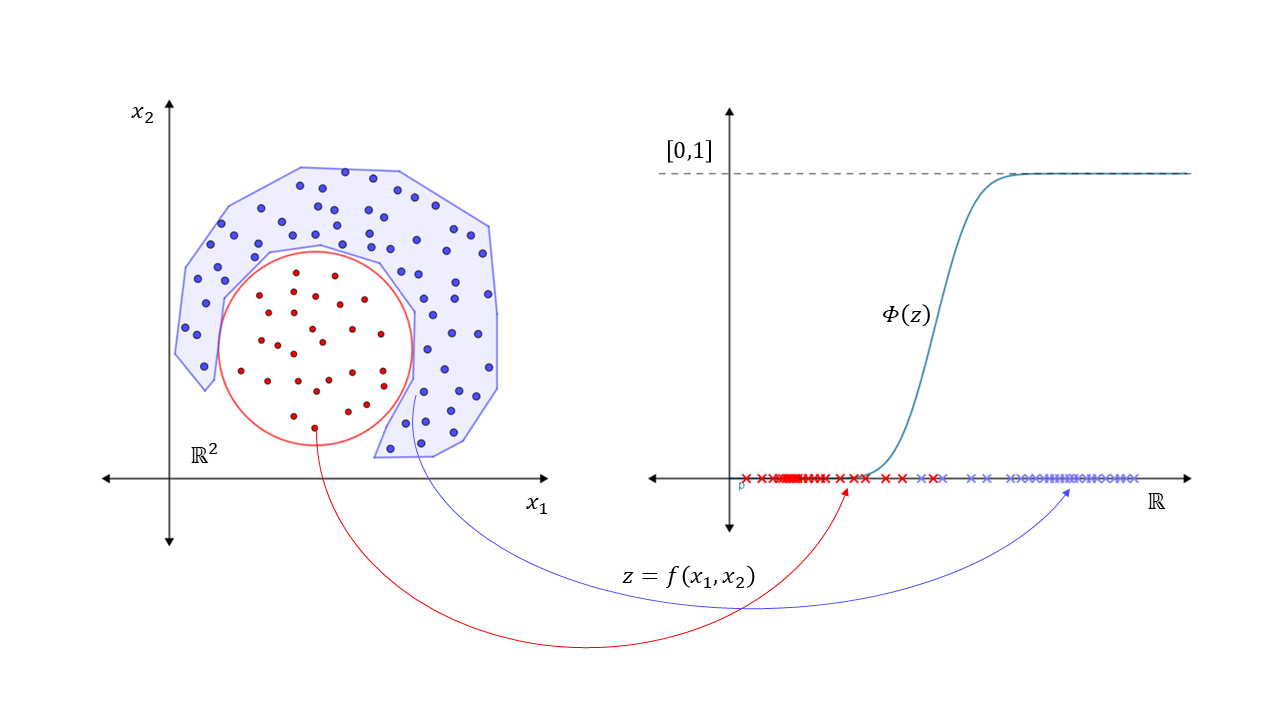
\includegraphics[width = 1\textwidth]{Diagrama_Separabilidad}
  \caption{Diagrama explicativo de un modelo de clasificación probit no lineal}
  \label{fig:DiagramaIntro}
\end{figure}

% De donde y cómo? Estructura del modelo - Cap. 2
Se comienza con una discusión teórica en el capítulo \ref{cap:Modelo} donde se presentan los conceptos que irán constuyendo al modelo. Primeramente se estudian los modelos lineales generalizados (GLM),  específicamente los modelos probit. Los GLM como su nombre lo indica, generalizan las regresiones tradicionales donde la respuesta $y_i$ es escalar ($y_i \in \mathbb{R}$) a regresiones donde la respuesta puede ser discreta o restringida a cierto dominio \autocite{maccullagh1989generalized}. No obstante, los GLM siguen siendo lineales en covariables pero se pueden flexibilizar usando diversas técnicas; entre ellas, los modelos aditivos generalizados (GAM) presentados en \citet{hastie1986generalized}. En estos modelos, la flexibilización se logra al transformar las covariables $\xni$ mediante una función de predicción $\eta$, usando métodos no paramétricos con base en suavizadores. Para este trabajo, se toman esos conceptos y se mezclan con los de \citet{mallik1998automatic} los cuales optan por darle una forma funcional concreta a $\eta$, correspondiente a una expansión de bases funcionales, particularmente, en polinomios por partes de continuidad y grado arbitrarios.  Asimismo, a lo largo del capítulo se verá que los conceptos mostrados abren las posibilidades en cuanto a modelos y datos sobre los que se puede hacer inferencia. Para finalizar el capítulo, se define una versión preliminar del modelo. %La expansión resultante, tiene la peculiaridad que conectan muchas disciplinas y ramas de las matemáticas que han sido de mucha utilidad no sólo en el campo de la estadística.

% Paradigma Bayesiano - Cap. 3
Para complementar la formulación funcional previa, el capítulo \ref{cap:BayesAlgoritmo} introduce de forma breve las ideas de la escuela bayesiana de la estadística, en particular el apredizaje bayesiano bajo un contexto de regresión. Este paradigma, responde a que bajo el trabajo de \citet{albert1993bayesian}, el modelo se puede plantear de tal forma que el algoritmo de aprendizaje se induce de forma natural. Para ello, se debe estudiar el muestreo de Gibbs que recae sobre otros conceptos fundamentales de la estadística bayesiana. Asimismo, el paradigma bayesiano resuena con las ideas del autor en cuanto a lo que implica la probabilidad como una forma de \emph{medir la incertidumbre} y la actualización del conocimiento.

% Modelo en si y algoritmo - Cap 4
Motivado por los conceptos del aprendizaje bayesiano, el capítulo \ref{cap:bpwpm} especifica en su forma final el modelo el cual se titula \emph{bpwpm} por las siglas en inglés de \textit{bayesian piecewise polinomial model}. Asimismo, el capítulo presenta en su forma más completa el algoritmo de aprendizaje usado para la estimación de los parámetros. Esta implementación se realiza a través de un paquete del mismo nombre desarrollado en el lenguaje abierto de programación estadística \verb|R|.\footnote{El desarrollo y explicación del paquete de cómputo se detalla en el apéndice \ref{ap:Paquete}. El paquete se puede descargar libremente de: \url{https://github.com/PaoloLuciano/bpwpm}. Asimismo, en la página \ref{tab:Codigo} se presenta un ejemplo mínimo funcional para que el lector pueda poner el modelo a prueba.}

% Cómo se probo? Cap. 5
En el capítulo \ref{cap:EjYRes} el modelo se prueba y se valida haciendo inferencia sobre seis bases de datos. No obstante, primero se hace una breve discusión sobre cómo evaluar la efectividad y precisión de un modelo como el presentado en este trabajo. Posteriormente, se estiman los parámetros del modelo en cinco bases de datos simuladas, todas con dos covariables ($\xsn_i \in \mathbb{R}^2$). Estas pruebas preliminares sirven para demostrar las capacidades predictivas del modelo y sobre todo, para hacer más concretas las matemáticas subyacentes, además de poder visualizar las diferentes fronteras flexibles obtenidas por el modelo. Asimismo, en este capítulo se discute la convergencia de las cadenas obtenidas por el muestreador de Gibbs. Para cerrar el capítulo, se replica un escenario real de análisis y modelado usando una base de datos médicos de cáncer.

% Y luego? Conclusión Cap. 6
Para terminar el trabajo, el capítulo \ref{cap:Conclusiones} abre la discusión sobre las limitantes del modelo y se presentan las consideraciones finales. Sin embargo, también discuten las múltiples posibles extensiones para mejorarlo. Posteriormente, se da un rápido vistazo a modelos relativamente más modernos los cuales han sido capaces de proezas computacionales que se creían imposibles hace algunas décadas. No obstante, se verá que muchos de estos modelos más complejos son generalizaciones de modelos clásicos y extensiones análogas del trabajo presentado. 
\end{document}